% -*- mode: latex; TeX-master: "Vorbis_I_spec"; -*-
%!TEX root = Vorbis_I_spec.tex
% $Id$
\section{Introduction and Description} \label{vorbis:spec:intro}

\subsection{Overview}

This document provides a high level description of the Vorbis codec's
construction.  A bit-by-bit specification appears beginning in
\xref{vorbis:spec:codec}.
The later sections assume a high-level
understanding of the Vorbis decode process, which is
provided here.

\subsubsection{Application}
Vorbis is a general purpose perceptual audio CODEC intended to allow
maximum encoder flexibility, thus allowing it to scale competitively
over an exceptionally wide range of bitrates.  At the high
quality/bitrate end of the scale (CD or DAT rate stereo, 16/24 bits)
it is in the same league as MPEG-2 and MPC.  Similarly, the 1.0
encoder can encode high-quality CD and DAT rate stereo at below 48kbps
without resampling to a lower rate.  Vorbis is also intended for
lower and higher sample rates (from 8kHz telephony to 192kHz digital
masters) and a range of channel representations (monaural,
polyphonic, stereo, quadraphonic, 5.1, ambisonic, or up to 255
discrete channels).


\subsubsection{Classification}
Vorbis I is a forward-adaptive monolithic transform CODEC based on the
Modified Discrete Cosine Transform.  The codec is structured to allow
addition of a hybrid wavelet filterbank in Vorbis II to offer better
transient response and reproduction using a transform better suited to
localized time events.


\subsubsection{Assumptions}

The Vorbis CODEC design assumes a complex, psychoacoustically-aware
encoder and simple, low-complexity decoder. Vorbis decode is
computationally simpler than mp3, although it does require more
working memory as Vorbis has no static probability model; the vector
codebooks used in the first stage of decoding from the bitstream are
packed in their entirety into the Vorbis bitstream headers. In
packed form, these codebooks occupy only a few kilobytes; the extent
to which they are pre-decoded into a cache is the dominant factor in
decoder memory usage.


Vorbis provides none of its own framing, synchronization or protection
against errors; it is solely a method of accepting input audio,
dividing it into individual frames and compressing these frames into
raw, unformatted 'packets'. The decoder then accepts these raw
packets in sequence, decodes them, synthesizes audio frames from
them, and reassembles the frames into a facsimile of the original
audio stream. Vorbis is a free-form variable bit rate (VBR) codec and packets have no
minimum size, maximum size, or fixed/expected size.  Packets
are designed that they may be truncated (or padded) and remain
decodable; this is not to be considered an error condition and is used
extensively in bitrate management in peeling.  Both the transport
mechanism and decoder must allow that a packet may be any size, or
end before or after packet decode expects.

Vorbis packets are thus intended to be used with a transport mechanism
that provides free-form framing, sync, positioning and error correction
in accordance with these design assumptions, such as Ogg (for file
transport) or RTP (for network multicast).  For purposes of a few
examples in this document, we will assume that Vorbis is to be
embedded in an Ogg stream specifically, although this is by no means a
requirement or fundamental assumption in the Vorbis design.

The specification for embedding Vorbis into
an Ogg transport stream is in \xref{vorbis:over:ogg}.



\subsubsection{Codec Setup and Probability Model}

Vorbis' heritage is as a research CODEC and its current design
reflects a desire to allow multiple decades of continuous encoder
improvement before running out of room within the codec specification.
For these reasons, configurable aspects of codec setup intentionally
lean toward the extreme of forward adaptive.

The single most controversial design decision in Vorbis (and the most
unusual for a Vorbis developer to keep in mind) is that the entire
probability model of the codec, the Huffman and VQ codebooks, is
packed into the bitstream header along with extensive CODEC setup
parameters (often several hundred fields).  This makes it impossible,
as it would be with MPEG audio layers, to embed a simple frame type
flag in each audio packet, or begin decode at any frame in the stream
without having previously fetched the codec setup header.


\begin{note}
Vorbis \emph{can} initiate decode at any arbitrary packet within a
bitstream so long as the codec has been initialized/setup with the
setup headers.
\end{note}

Thus, Vorbis headers are both required for decode to begin and
relatively large as bitstream headers go.  The header size is
unbounded, although for streaming a rule-of-thumb of 4kB or less is
recommended (and Xiph.Org's Vorbis encoder follows this suggestion).

Our own design work indicates the primary liability of the
required header is in mindshare; it is an unusual design and thus
causes some amount of complaint among engineers as this runs against
current design trends (and also points out limitations in some
existing software/interface designs, such as Windows' ACM codec
framework).  However, we find that it does not fundamentally limit
Vorbis' suitable application space.


\subsubsection{Format Specification}
The Vorbis format is well-defined by its decode specification; any
encoder that produces packets that are correctly decoded by the
reference Vorbis decoder described below may be considered a proper
Vorbis encoder.  A decoder must faithfully and completely implement
the specification defined below (except where noted) to be considered
a proper Vorbis decoder.

\subsubsection{Hardware Profile}
Although Vorbis decode is computationally simple, it may still run
into specific limitations of an embedded design.  For this reason,
embedded designs are allowed to deviate in limited ways from the
`full' decode specification yet still be certified compliant.  These
optional omissions are labelled in the spec where relevant.


\subsection{Decoder Configuration}

Decoder setup consists of configuration of multiple, self-contained
component abstractions that perform specific functions in the decode
pipeline.  Each different component instance of a specific type is
semantically interchangeable; decoder configuration consists both of
internal component configuration, as well as arrangement of specific
instances into a decode pipeline.  Componentry arrangement is roughly
as follows:

\begin{center}
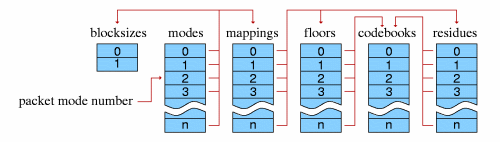
\includegraphics[width=\textwidth]{components}
\captionof{figure}{decoder pipeline configuration}
\end{center}

\subsubsection{Global Config}
Global codec configuration consists of a few audio related fields
(sample rate, channels), Vorbis version (always '0' in Vorbis I),
bitrate hints, and the lists of component instances.  All other
configuration is in the context of specific components.

\subsubsection{Mode}

Each Vorbis frame is coded according to a master 'mode'.  A bitstream
may use one or many modes.

The mode mechanism is used to encode a frame according to one of
multiple possible methods with the intention of choosing a method best
suited to that frame.  Different modes are, e.g. how frame size
is changed from frame to frame. The mode number of a frame serves as a
top level configuration switch for all other specific aspects of frame
decode.

A 'mode' configuration consists of a frame size setting, window type
(always 0, the Vorbis window, in Vorbis I), transform type (always
type 0, the MDCT, in Vorbis I) and a mapping number.  The mapping
number specifies which mapping configuration instance to use for
low-level packet decode and synthesis.


\subsubsection{Mapping}

A mapping contains a channel coupling description and a list of
'submaps' that bundle sets of channel vectors together for grouped
encoding and decoding. These submaps are not references to external
components; the submap list is internal and specific to a mapping.

A 'submap' is a configuration/grouping that applies to a subset of
floor and residue vectors within a mapping.  The submap functions as a
last layer of indirection such that specific special floor or residue
settings can be applied not only to all the vectors in a given mode,
but also specific vectors in a specific mode.  Each submap specifies
the proper floor and residue instance number to use for decoding that
submap's spectral floor and spectral residue vectors.

As an example:

Assume a Vorbis stream that contains six channels in the standard 5.1
format.  The sixth channel, as is normal in 5.1, is bass only.
Therefore it would be wasteful to encode a full-spectrum version of it
as with the other channels.  The submapping mechanism can be used to
apply a full range floor and residue encoding to channels 0 through 4,
and a bass-only representation to the bass channel, thus saving space.
In this example, channels 0-4 belong to submap 0 (which indicates use
of a full-range floor) and channel 5 belongs to submap 1, which uses a
bass-only representation.


\subsubsection{Floor}

Vorbis encodes a spectral 'floor' vector for each PCM channel.  This
vector is a low-resolution representation of the audio spectrum for
the given channel in the current frame, generally used akin to a
whitening filter.  It is named a 'floor' because the Xiph.Org
reference encoder has historically used it as a unit-baseline for
spectral resolution.

A floor encoding may be of two types.  Floor 0 uses a packed LSP
representation on a dB amplitude scale and Bark frequency scale.
Floor 1 represents the curve as a piecewise linear interpolated
representation on a dB amplitude scale and linear frequency scale.
The two floors are semantically interchangeable in
encoding/decoding. However, floor type 1 provides more stable
inter-frame behavior, and so is the preferred choice in all
coupled-stereo and high bitrate modes.  Floor 1 is also considerably
less expensive to decode than floor 0.

Floor 0 is not to be considered deprecated, but it is of limited
modern use.  No known Vorbis encoder past Xiph.Org's own beta 4 makes
use of floor 0.

The values coded/decoded by a floor are both compactly formatted and
make use of entropy coding to save space.  For this reason, a floor
configuration generally refers to multiple codebooks in the codebook
component list.  Entropy coding is thus provided as an abstraction,
and each floor instance may choose from any and all available
codebooks when coding/decoding.


\subsubsection{Residue}
The spectral residue is the fine structure of the audio spectrum
once the floor curve has been subtracted out.  In simplest terms, it
is coded in the bitstream using cascaded (multi-pass) vector
quantization according to one of three specific packing/coding
algorithms numbered 0 through 2.  The packing algorithm details are
configured by residue instance.  As with the floor components, the
final VQ/entropy encoding is provided by external codebook instances
and each residue instance may choose from any and all available
codebooks.

\subsubsection{Codebooks}

Codebooks are a self-contained abstraction that perform entropy
decoding and, optionally, use the entropy-decoded integer value as an
offset into an index of output value vectors, returning the indicated
vector of values.

The entropy coding in a Vorbis I codebook is provided by a standard
Huffman binary tree representation.  This tree is tightly packed using
one of several methods, depending on whether codeword lengths are
ordered or unordered, or the tree is sparse.

The codebook vector index is similarly packed according to index
characteristic.  Most commonly, the vector index is encoded as a
single list of values of possible values that are then permuted into
a list of n-dimensional rows (lattice VQ).



\subsection{High-level Decode Process}

\subsubsection{Decode Setup}

Before decoding can begin, a decoder must initialize using the
bitstream headers matching the stream to be decoded.  Vorbis uses
three header packets; all are required, in-order, by this
specification. Once set up, decode may begin at any audio packet
belonging to the Vorbis stream. In Vorbis I, all packets after the
three initial headers are audio packets.

The header packets are, in order, the identification
header, the comments header, and the setup header.

\paragraph{Identification Header}
The identification header identifies the bitstream as Vorbis, Vorbis
version, and the simple audio characteristics of the stream such as
sample rate and number of channels.

\paragraph{Comment Header}
The comment header includes user text comments (``tags'') and a vendor
string for the application/library that produced the bitstream.  The
encoding and proper use of the comment header is described in \xref{vorbis:spec:comment}.

\paragraph{Setup Header}
The setup header includes extensive CODEC setup information as well as
the complete VQ and Huffman codebooks needed for decode.


\subsubsection{Decode Procedure}

The decoding and synthesis procedure for all audio packets is
fundamentally the same.
\begin{enumerate}
\item decode packet type flag
\item decode mode number
\item decode window shape (long windows only)
\item decode floor
\item decode residue into residue vectors
\item inverse channel coupling of residue vectors
\item generate floor curve from decoded floor data
\item compute dot product of floor and residue, producing audio spectrum vector
\item inverse monolithic transform of audio spectrum vector, always an MDCT in Vorbis I
\item overlap/add left-hand output of transform with right-hand output of previous frame
\item store right hand-data from transform of current frame for future lapping
\item if not first frame, return results of overlap/add as audio result of current frame
\end{enumerate}

Note that clever rearrangement of the synthesis arithmetic is
possible; as an example, one can take advantage of symmetries in the
MDCT to store the right-hand transform data of a partial MDCT for a
50\% inter-frame buffer space savings, and then complete the transform
later before overlap/add with the next frame.  This optimization
produces entirely equivalent output and is naturally perfectly legal.
The decoder must be \emph{entirely mathematically equivalent} to the
specification, it need not be a literal semantic implementation.

\paragraph{Packet type decode}

Vorbis I uses four packet types. The first three packet types mark each
of the three Vorbis headers described above. The fourth packet type
marks an audio packet. All other packet types are reserved; packets
marked with a reserved type should be ignored.

Following the three header packets, all packets in a Vorbis I stream
are audio.  The first step of audio packet decode is to read and
verify the packet type; \emph{a non-audio packet when audio is expected
indicates stream corruption or a non-compliant stream. The decoder
must ignore the packet and not attempt decoding it to
audio}.




\paragraph{Mode decode}
Vorbis allows an encoder to set up multiple, numbered packet 'modes',
as described earlier, all of which may be used in a given Vorbis
stream. The mode is encoded as an integer used as a direct offset into
the mode instance index.


\paragraph{Window shape decode (long windows only)} \label{vorbis:spec:window}

Vorbis frames may be one of two PCM sample sizes specified during
codec setup.  In Vorbis I, legal frame sizes are powers of two from 64
to 8192 samples.  Aside from coupling, Vorbis handles channels as
independent vectors and these frame sizes are in samples per channel.

Vorbis uses an overlapping transform, namely the MDCT, to blend one
frame into the next, avoiding most inter-frame block boundary
artifacts.  The MDCT output of one frame is windowed according to MDCT
requirements, overlapped 50\% with the output of the previous frame and
added.  The window shape assures seamless reconstruction.

This is easy to visualize in the case of equal sized-windows:

\begin{center}
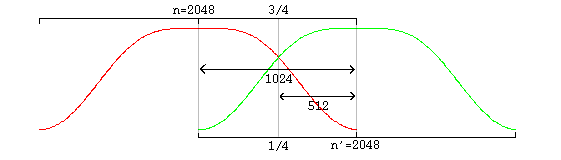
\includegraphics[width=\textwidth]{window1}
\captionof{figure}{overlap of two equal-sized windows}
\end{center}

And slightly more complex in the case of overlapping unequal sized
windows:

\begin{center}
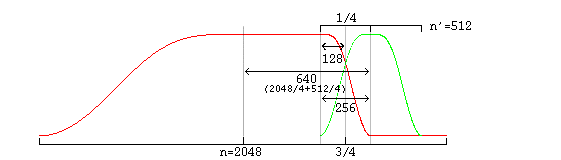
\includegraphics[width=\textwidth]{window2}
\captionof{figure}{overlap of a long and a short window}
\end{center}

In the unequal-sized window case, the window shape of the long window
must be modified for seamless lapping as above.  It is possible to
correctly infer window shape to be applied to the current window from
knowing the sizes of the current, previous and next window.  It is
legal for a decoder to use this method. However, in the case of a long
window (short windows require no modification), Vorbis also codes two
flag bits to specify pre- and post- window shape.  Although not
strictly necessary for function, this minor redundancy allows a packet
to be fully decoded to the point of lapping entirely independently of
any other packet, allowing easier abstraction of decode layers as well
as allowing a greater level of easy parallelism in encode and
decode.

A description of valid window functions for use with an inverse MDCT
can be found in \cite{Sporer/Brandenburg/Edler}.  Vorbis windows
all use the slope function
\[ y = \sin(.5*\pi \, \sin^2((x+.5)/n*\pi)) . \]



\paragraph{floor decode}
Each floor is encoded/decoded in channel order, however each floor
belongs to a 'submap' that specifies which floor configuration to
use.  All floors are decoded before residue decode begins.


\paragraph{residue decode}

Although the number of residue vectors equals the number of channels,
channel coupling may mean that the raw residue vectors extracted
during decode do not map directly to specific channels.  When channel
coupling is in use, some vectors will correspond to coupled magnitude
or angle.  The coupling relationships are described in the codec setup
and may differ from frame to frame, due to different mode numbers.

Vorbis codes residue vectors in groups by submap; the coding is done
in submap order from submap 0 through n-1.  This differs from floors
which are coded using a configuration provided by submap number, but
are coded individually in channel order.



\paragraph{inverse channel coupling}

A detailed discussion of stereo in the Vorbis codec can be found in
the document \href{stereo.html}{Stereo Channel Coupling in the
Vorbis CODEC}.  Vorbis is not limited to only stereo coupling, but
the stereo document also gives a good overview of the generic coupling
mechanism.

Vorbis coupling applies to pairs of residue vectors at a time;
decoupling is done in-place a pair at a time in the order and using
the vectors specified in the current mapping configuration.  The
decoupling operation is the same for all pairs, converting square
polar representation (where one vector is magnitude and the second
angle) back to Cartesian representation.

After decoupling, in order, each pair of vectors on the coupling list,
the resulting residue vectors represent the fine spectral detail
of each output channel.



\paragraph{generate floor curve}

The decoder may choose to generate the floor curve at any appropriate
time.  It is reasonable to generate the output curve when the floor
data is decoded from the raw packet, or it can be generated after
inverse coupling and applied to the spectral residue directly,
combining generation and the dot product into one step and eliminating
some working space.

Both floor 0 and floor 1 generate a linear-range, linear-domain output
vector to be multiplied (dot product) by the linear-range,
linear-domain spectral residue.



\paragraph{compute floor/residue dot product}

This step is straightforward; for each output channel, the decoder
multiplies the floor curve and residue vectors element by element,
producing the finished audio spectrum of each channel.

% TODO/FIXME: The following two paragraphs have identical twins
%   in section 4 (under "dot product")
One point is worth mentioning about this dot product; a common mistake
in a fixed point implementation might be to assume that a 32 bit
fixed-point representation for floor and residue and direct
multiplication of the vectors is sufficient for acceptable spectral
depth in all cases because it happens to mostly work with the current
Xiph.Org reference encoder.

However, floor vector values can span \~{}140dB (\~{}24 bits unsigned), and
the audio spectrum vector should represent a minimum of 120dB (\~{}21
bits with sign), even when output is to a 16 bit PCM device.  For the
residue vector to represent full scale if the floor is nailed to
$-140$dB, it must be able to span 0 to $+140$dB.  For the residue vector
to reach full scale if the floor is nailed at 0dB, it must be able to
represent $-140$dB to $+0$dB.  Thus, in order to handle full range
dynamics, a residue vector may span $-140$dB to $+140$dB entirely within
spec.  A 280dB range is approximately 48 bits with sign; thus the
residue vector must be able to represent a 48 bit range and the dot
product must be able to handle an effective 48 bit times 24 bit
multiplication.  This range may be achieved using large (64 bit or
larger) integers, or implementing a movable binary point
representation.



\paragraph{inverse monolithic transform (MDCT)}

The audio spectrum is converted back into time domain PCM audio via an
inverse Modified Discrete Cosine Transform (MDCT).  A detailed
description of the MDCT is available in \cite{Sporer/Brandenburg/Edler}.

Note that the PCM produced directly from the MDCT is not yet finished
audio; it must be lapped with surrounding frames using an appropriate
window (such as the Vorbis window) before the MDCT can be considered
orthogonal.



\paragraph{overlap/add data}
Windowed MDCT output is overlapped and added with the right hand data
of the previous window such that the 3/4 point of the previous window
is aligned with the 1/4 point of the current window (as illustrated in
the window overlap diagram). At this point, the audio data between the
center of the previous frame and the center of the current frame is
now finished and ready to be returned.


\paragraph{cache right hand data}
The decoder must cache the right hand portion of the current frame to
be lapped with the left hand portion of the next frame.



\paragraph{return finished audio data}

The overlapped portion produced from overlapping the previous and
current frame data is finished data to be returned by the decoder.
This data spans from the center of the previous window to the center
of the current window.  In the case of same-sized windows, the amount
of data to return is one-half block consisting of and only of the
overlapped portions. When overlapping a short and long window, much of
the returned range is not actually overlap.  This does not damage
transform orthogonality.  Pay attention however to returning the
correct data range; the amount of data to be returned is:

\begin{Verbatim}[commandchars=\\\{\}]
window\_blocksize(previous\_window)/4+window\_blocksize(current\_window)/4
\end{Verbatim}

from the center of the previous window to the center of the current
window.

Data is not returned from the first frame; it must be used to 'prime'
the decode engine.  The encoder accounts for this priming when
calculating PCM offsets; after the first frame, the proper PCM output
offset is '0' (as no data has been returned yet).
